% -*- TeX-master: "master.tex" -*-
\newcommand{\up}{\uparrow}
\newcommand{\dn}{\downarrow}
\section{Symmetry}
The study of symmetry has been a central theme in the study of physics. In 1917 Emmy Noether proved that (for a specific type of field-complex, 4-dimensional) a symmetry of the Hamiltonian implied the existence of a conserved quantity

You have studied the correspondence of symmetries and conserved quantities in classical and quantum mechanics:
\begin{itemize}
\item Time translation invariance $\iff$ Energy conservation
\item Space translation invariance $\iff$ Momentum conservation
\item Rotational invariance $\iff$ Angular momentum conservation
\end{itemize}

The construction of the Standard Model (and much of theoretical thought) has been largely the identification of the symmetries associated with observed conserved quantities.

\begin{aside}
  Not all conserved quantities must come from symmetries, e.g. solitons and other topological properties etc.
\end{aside}

A conserved quantity is one that is unchanged by a transformation, e.g. a Lorentz scalar under a Lorentz transformation.

The set of possible transformations of a given type have the properties of a \underline{group}. Hence, we study groups and algebras

\subsection{Group Theory}
Reminder of group definitions
\begin{enumerate}
\item Clousure: if $A\in G$, $B\in G$, then $AB\in G$
\item $\exists$ an identity: $I\in G$
\item Every element has an inverse: $A\in G$, $AA^{-1}=A^{-1}A=I$ with $A^{-1}\in G$
\item Associativity: $(AB)C=A(BC)$
\end{enumerate}

\subsubsection{Rotation Group}
Consider rotation by angle $\theta$ about the $z$-axis:
\begin{align*}
  \pmqty{x'\\y'\\z'}=
  \underbrace{\pmqty{\cos\theta & \sin\theta&\\
      -\sin\theta&\cos\theta&\\&&1}}_{R_z(\theta)}
  \pmqty{x\\y\\z}
\end{align*}
Similarly:
\begin{align*}
  R_x(\theta)=
  \pmqty{1\\&\cos\theta&\sin\theta\\&-\sin\theta&\cos\theta}
  \qquad
  R_y(\theta)=
  \pmqty{\cos\theta&&\sin\theta\\&1&\\-\sin\theta&&\cos\theta}
\end{align*}
Two successive rotations is also a rotation (closure). Can you quickly show the other group requirements?

Rotations leave the length of a vector invariant:
\begin{align*}
  (x')^2=x_i'x_i'=R_{ij}R_{ik}x_jx_k=(R^T)_{ji}R_{ik}x_jx_k=\delta_{jk}x_jx_k
  =x_kx_k=x^2
\end{align*}

So rotations form a three-dimensional orthogonal group, called $SO(3)$. In addition:
\begin{align*}
  \det{R}=\cos^2\theta+\sin^2\theta=1
\end{align*}
So the rotation group is $SO(3)$, S for special, O for orthogonal.

Recal the Lorentz group is $SO(3,1)$. Rotations are a \underline{subgroup} of the Lorentz Group:
\begin{align*}
  \Lambda^\mu_\nu=\pmqty{\text{Boosts}&\\&3\times3\text{ Rotations}}
\end{align*}
So the Lorentz group $=$ Boosts + Rotations

\subsubsection{Spin}
Consider a particle of mass $m$ at rest. Its four-momentum is:
\begin{align*}
  p^\mu=\pmqty{m\\0\\0\\0}
\end{align*}
Certainly the particle's four-momentum is invariant under rotations. The spin of the particle tells you how the wavefunction of the particle transforms  under the rotation group:
\begin{itemize}
\item Spin 0: $R=\bm{1}$ Trivial
\item Spin $\frac12$: $R_i=\exp{i\frac12\theta_i\sigma_i}$ where $\sigma_i$ are the Pauli matrices $(2\times2)$
\item Spin 1: $R=3\times3$ Rotation matrices (see above)
\item Spin $\frac32$: $R=4\times4$ matrices
\item Spin $j$: $R=(2j+1)\times(2j+1)$ matrices
\end{itemize}
So the spin of a particle is related to its \underline{representation} of the rotation group

Formally, a representation is a homomorphic mapping of a group onto the matrices $(GL_n)$ of rank $n$.

The symmetry associated with rotations is continuous. Hence, rather than work directly with the rotation matrices, we may work with the significantly simpler infinitesimal roations:

Let $R(\theta)=\exp{i\theta_iT_i}\equiv e^{i\theta_iT_i}$, where $T_i$ are matrices, $i=x,y,z$, and $\exp$ of a matrix is just the shorthand for:
\begin{align*}
  \exp{M}=e^M\equiv\sum_{i=0}^\infty\frac{M^n}{n!}
\end{align*}
We know that $R^TR\equiv\bm{1}$, so that $\exp{i\theta_iT_i}^T\exp{i\theta_iT_i}=\bm{1}$. Consider $\theta_i$ to be infinitesimal and expand:
\begin{align*}
  (\bm{1}+i\theta_iT_i^T+\cdots)
  (\bm{1}+i\theta_iT_i^T+\cdots)&=\bm{1}\\
  \implies \theta_i\qty[T_i^T+T_i]&=0
\end{align*}
Thus we arrive at $T_i^T=-T_i$, that is, $T_i$ are \underline{antisymmetric matrices}.

Consider: $R_x(\theta)$ with $\theta\ll 1$:
\begin{align*}
  R_x(\theta\ll1)&=\pmqty{1\\&1&-\theta\\&\theta&1}\\
  &=\bm{1}+\theta\pmqty{0&0&0\\0&0&-1\\0&1&0}
\end{align*}
From above, we can then identify $iT_x$ as this second matrix. Repeating the above process for $R_y,R_z$, we obtain a full set of generators of $SO(3)$:
\begin{align*}
  iT_x=\pmqty{0&0&0\\0&0&-1\\0&1&0}\quad
  iT_y=\pmqty{0&0&-1\\0&0&0\\1&0&0}\quad
  iT_z=\pmqty{0&-1&0\\1&0&0\\0&0&0}
\end{align*}

Consider two successive rotations:
\begin{gather*}
  R(\theta)R(\theta')=R(\theta'')\\
  R(\theta)=\bm{1}+i\theta\vdot T
\end{gather*}
Since they form a group, the right hand side should also be a rotation, and we have our definition of the generator below, with $\theta\vdot T=\theta_iT_i$. Plugging this form into the above:
\begin{align*}
  (\bm{1}+i\theta\vdot T+\frac12(i\theta\vdot T)^2+\cdots)
  (\bm{1}+i\theta'\vdot T+\frac12(i\theta'\vdot T)^2+\cdots)=
  (\bm{1}+i\theta''\vdot T+\frac12(i\theta''\vdot T)^2+\cdots)
\end{align*}
This gives you that $\theta+\theta'=\theta''$ to first order, $\order{\theta}$. If we go to second order, we would find that $\theta+\theta'=\theta''+\alpha$ where $\alpha\sim\order{\theta^2}$. Here we find that:
\begin{align*}
  -\frac12\qty[(\theta\vdot T)^2+(\theta'\vdot T)^2+2(\theta\vdot T)(\theta'\vdot T)]=-\frac12\qty[(\theta''\vdot T)^2-2i\alpha\vdot T]
\end{align*}
Now the second order term will tell us:
\begin{align*}
  (\theta''\vdot T)^2=\qty[\theta\vdot T+\theta'\vdot T-\alpha\vdot T]^2
\end{align*}
However we can essentially ignore the $\alpha\vdot T$ cross terms since all the other terms are at least order $\theta$, and the resulting multiplied term would be $\order{\theta^3}$ or greater, which we do not need to consider. Hence we find:
\begin{align*}
  (\theta''\vdot T)^2=(\theta\vdot T)^2+(\theta'\vdot T)^2+(\theta'\vdot T)(\theta\vdot T)+(\theta\vdot T)(\theta'\vdot T)
\end{align*}
This gives a relation between $\alpha$ and the other second order terms:
\begin{align*}
  -2i\alpha\vdot T=
  (\theta\vdot T)(\theta'\vdot T)-(\theta'\vdot T)(\theta\vdot T)
\end{align*}
Since $\alpha\sim\order{\theta^2}$, and for the above equation to hold it must be proportional to $\theta\theta'$. Let $\alpha_i\equiv-\frac12f_{jki}\theta_jtheta'_k$. We then find:
\begin{align*}
  if_{jki}\theta_j\theta'_kT_i&=\theta_j\theta'_k\qty[T_jT_k-T_kT_j]\\
  \implies if_{jki}T_i=T_jT_k-T_kT_j
\end{align*}
Define the commutator: $\comm{A}{B}\equiv AB-BA$, so that we can relabel:
\begin{align*}
  \boxed{\comm{T_i}{T_j}=if_{ijk}T_k}
\end{align*}
From this we find $f_{ijk}=-f_{jik}$. These are called structure constants, and are real valued.

This commutator above tells us that $SO(3)$ is a \underline{Lie Group}, i.e. a continuous group (on a differentiable manifold).

The generators $T_i$ of $SO(3)$ form a \underline{graded Lie algebra} with structure constants $f_{ijk}$

The structure constants for $SO(3)$ are $f_{ijk}=\veps_{ijk}$, with $\veps_{123}=+1$, the totally antisymmetric tensor. In other words the commutators are given as:
\begin{align*}
  \comm{T_x}{T_y}&=iT_z\\
  \comm{T_y}{T_z}&=iT_x\\
  \comm{T_z}{T_x}&=iT_y
\end{align*}

A \underline{representation} of the $SO(3)$ Lie algebra is any set of matrices which satisfy
\begin{align*}
  \comm{T_i}{T_j}=i\veps_{ijk}T_k
\end{align*}
The $3\times 3$ matrices we have written are called the \underline{fundamental representation} (also known as the \underline{defining representation}).

Recal this was associated with spin-1 particles.

\subsection{Spin $\frac12$ Representation}
The generators associated with spin-$\frac12$ are:
\begin{align*}
  T_x=\frac12\pmqty{&1\\1&}\quad
  T_y=\frac12\pmqty{&i\\-i&}\quad
  T_z=\frac12\pmqty{1& \\ &-1}
\end{align*}
Which are related to the Pauli Matrices, i.e. $T_i=\frac12\sigma_i$.

One can show that these $2\times 2$ matrices $T_i$ satisfy $\comm{T_i}{T_j}=i\veps_{ijk}T_k$, so they do form a representation of $SO(3)$.

The $T_i$ for this representation are \underline{not} antisymmetric, but they are Hermitian:
\begin{align*}
  T_i^\dag=T_i
\end{align*}
The rotation matrices $R=\exp{iT}$ are therefore \underline{unitary}:
\begin{align*}
  R^\dag R=(e^{iT})^\dag e^{iT}=e^{-iT^\dag}e^{iT}=e^{-iT}e^{iT}=\bm{1}
\end{align*}
To emphasize this, let's call these $2\times2$ matrices $U$ instead of $R$, so:
\begin{align*}
  U^\dag U=\bm{1}
\end{align*}

These $2\times2$ complex, unitary rotation matrices represent the group $SO(3)$, \underline{but} they also represent the group $SU(2)$, where $SU(2)$ means \textbf{s}pecial (determinant 1) \textbf{u}nitary $\mathbf{2\times2}$ matrices.
\begin{aside}
  Note that $\det U$ can be shown to be $1$:
  \begin{align*}
    \det U=\det e^{iT}=\exp{i\Tr[T]}=e^{i0}=1
  \end{align*}
  Since $T$ are traceless in general.
\end{aside}

So we have proven the groups $SU(2)$ and $SO(3)$ have the \underline{same} Lie algebra. Thus the groups are identical as far as ``small'' rotations are concerned:
\begin{align*}
  SU(2)\underbrace{\approxeq}_{\text{Isomorphic}} SO(3)
\end{align*}

While the $3\times3$ $SO(3)$ matrices act on ordinary space $(x,y,z)$, the $2\times2$ complex $SU(2)$ matrices act on a complex, 2-dimensional ``spin'' space. We call this the \underline{fundamental} representation of $SU(2)$, but the \underline{spinor} representation of $SO(3)$.
\begin{remark}
  The so-called \underline{Classical Lie Groups} are $SO(n+1)$, $SU(n)$, and $SP(n+1)$, with the $p$ for symplectic. Some exceptions to these are $G_2, F_4, E_6, E_7, E_8$.

  It is also important to note that $SO(2)\approxeq U(1)$, so 2D rotations are equivalent to unitary numbers $e^{i\theta}$
\end{remark}

\subsection{Isospin}
Isospin (or Isotropic spin) is the symmetry of the strong interaction (QCD):
\begin{figure}[H]
  \centering
  \begin{tikzpicture}[scale=2.0]
    \begin{feynhand}
      % vertices
      \vertex (p11) at (1.5,0.5) {$u$};
      \vertex (p12) at (1.5,-0.5) {$\bar{u}$};
      \vertex (a1) at (0,0) {$g$};
      \vertex (b1) at (1,0);
      % propagators
      \propag [gluon] (a1) to (b1);
      \propag (b1) to (p11);
      \propag (b1) to (p12);
      \vertex (eq) at (1.75,0) {=};
      % vertices
      \vertex (p21) at (3.5,0.5) {$d$};
      \vertex (p22) at (3.5,-0.5) {$\bar{d}$};
      \vertex (a2) at (2,0) {$g$};
      \vertex (b2) at (3,0);
      % propagators
      \propag [gluon] (a2) to (b2);
      \propag (b2) to (p21);
      \propag (b2) to (p22);
    \end{feynhand}
  \end{tikzpicture}
  \caption{Isospin Conservation in QCD}
  \label{fig:isospin}
\end{figure}
So in QCD, $u$ and $d$ are interchangeable. This is the reason for isospin.

But, recall that $m_u\neq m_d$. So how is it possible that we can interchange $u$ and $d$?
\begin{figure}[H]
  \centering
  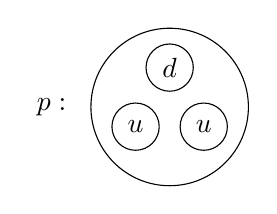
\begin{tikzpicture}
    \node at (0,0) {$p:$};
    \draw (1.500, 0.00) circle (1.0);
    \draw (1.500, 0.50) circle (0.3) node {$d$};
    \draw (1.067,-0.25) circle (0.3) node {$u$};
    \draw (1.933,-0.25) circle (0.3) node {$u$};
  \end{tikzpicture}
  \caption{Proton representation}
  \label{fig:proton}
\end{figure}
Recall the structure of the proton, and that $m_p\gg m_u,m_d$, this is because the proton mass is ``dynamical'' and is not due to the quark masses. So isospin is a good symmetry due to this difference in proton and up/down masses.

In group theory terms, we say that $\pmqty{u\\d}$ transform as a doublet under $SU(2)$ isospin

\begin{remark}
  \underline{\textbf{WARNING}}: $SU(2)$ ``isospin'' has nothing to do with $SU(2)$ spin! The mathematics is the same, but the physics is entirely different!
\end{remark}
One consequence of isospin is that $m_p=m_n$, this means that $\pmqty{p\\n}$ transform as an isospin doublet:
\begin{figure}[H]
  \centering
  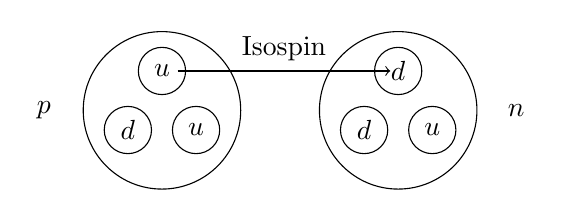
\begin{tikzpicture}
    \node at (0,0) {$p$};
    \draw (1.500, 0.00) circle (1.0);
    \draw (1.500, 0.50) circle (0.3) node {$u$};
    \draw (1.067,-0.25) circle (0.3) node {$d$};
    \draw (1.933,-0.25) circle (0.3) node {$u$};
    \node at (6,0) {$n$};
    \draw (4.500, 0.00) circle (1.0);
    \draw (4.500, 0.50) circle (0.3) node {$d$};
    \draw (4.067,-0.25) circle (0.3) node {$d$};
    \draw (4.933,-0.25) circle (0.3) node {$u$};
    \draw[->] (1.700, 0.500) -- (4.400, 0.500);
    \node at  (3.050, 0.500) [above] {Isospin};
  \end{tikzpicture}
  \caption{Proton \& Neutron in Isospin}
  \label{fig:isospinpn}
\end{figure}
Historically, this was the motivation for Heisenberg to suggest isospin differentiated ``nucleons,'' like $s_z=\pm\frac12$ differentiates the degeneracy in spin $\frac12$ systems.
\begin{note}
  The nuclear physicists use the much better term ``isobaric'' spin.

  E.g., Mirror nuclei, like $^7_3$Li/$^7_4$Be and $^{11}_5$B/$^{11}_6$C have nearly identical binding energies (after correcting for coulomb interaction)
\end{note}

\begin{definition}[Antiquarks]
  The so called antiquarks $\bar{u}$ and $\bar{d}$ are simply defined to be the complex conjugate of $u,d$.

  In group theory, this corresponds to $T_i$ representating the same algebra as $-T_i^*$:
  \begin{align*}
    \comm{T_i}{T_j}&=if_{ijk}T_k\\
    \comm{T_i^*}{T_j^*}&=-if_{ijk}T_k^*\\
    \implies\comm{(-T_i^*)}{(-T_j^*)}&=if_{ijk}(-T_k^*)
  \end{align*}
\end{definition}

For $SU(2)$, the complex conjugate representation is unitarily equivalent to the original representation:
\begin{align*}
  \underbrace{\pmqty{&-1\\1}}_{U}\qty(-T_i^*)
  \underbrace{\pmqty{&1\\-1}}_{U^\dag}=T_i
\end{align*}
For $T_i$ in the spin $\frac12$ representation, the representation is \underline{pseudoreal}.

Antiquarks transform as the c.c. rep., called the $\bar{2}$ representation:
\begin{align*}
  -T_i^*\pmqty{\bar{u}\\\bar{d}}&=\pmqty{\bar{u}'\\\bar{d}'}\\
  T_i\pmqty{-\bar{d}\\\bar{u}}&=\pmqty{-\bar{d}\\\bar{u}}
\end{align*}
Therefore, we can say that instead of using complex conjugate versions of the same algebra, we can use the usual spin-$\frac12$, instead on $\pmqty{-\bar{d}\\\bar{u}}$
\begin{definition}[Pions]
  Pions (or more generally mesons) are pairs of $q\bar{q}$, quarks and antiquarks.
\end{definition}
The strong interaction (QCD) not only binds quarks into $p,n$, it also binds quarks with antiquarks into \underline{pions}.

\begin{figure}[H]
  \centering
  
  \caption{Pion definition}
  \label{fig:pion}
\end{figure}
The charge of the pion is given by the sum of the charges of the $u$ and $\bar{d}$ quarks, that is $+\frac23+\frac13=1$.

In particular, pions are formed from the product of $\pmqty{u\\d}$ and $\pmqty{-\bar{d}\\u}$ isospin doublets. These are combined in the same way that we add spins:
\begin{example}[Adding Spins]
  Adding 2 spin-$\frac12$ particles, we have the following:
  \begin{align*}
    &\ket{J,J_z}\\
    &\ket{1, 1}=\ket{\up\up}\\
    &\ket{1, 0}
    =\frac1{\sqrt{2}}\qty(\ket{\up\dn}+\ket{\dn\up})\\
    &\ket{1,-1}=\ket{\dn\dn}\\
    &\ket{0,0}
    =\frac1{\sqrt{2}}\qty(\ket{\up\dn}-\ket{\dn\up})
  \end{align*}
  The first 3 are the spin 1 triplet, and the last 1 is the spin 0 singlet
\end{example}
\begin{example}[Adding IsoSpins]
  The math is exactly the same, except instead of $\up/\dn$ we will have $u,\bar{u},d,-\bar{d}$
  \begin{align*}
    &\ket{I,I_3}\\
    &\ket{1, 1}=\ket{u(-\bar{d})}\equiv\pi^+\\
    &\ket{1, 0}=\frac1{\sqrt{2}}\qty(\ket{u\bar{u}+d(-\bar{d})})\equiv\pi^0\\
    &\ket{1,-1}=\ket{d\bar{u}}\equiv\pi^-\\
    &\ket{0,0}=\frac1{\sqrt{2}}\qty(\ket{u\bar{u}-d(-\bar{d})})\equiv???
  \end{align*}
  The first 3 are the isospin 1 triplet, the pions, and the last is different, we will come back to it
\end{example}
So, we have isospin doublets of $\pmqty{p\\n}$ and $\pmqty{-n\\p}$, and the isospin triplet of $\pmqty{\pi^+\\\pi^0\\\pi^-}$. The pion masses are:
\begin{align*}
  m_{\pi^\pm}&=\SI{139.56}{\mega\eV}\\
  m_{\pi^0}&=\SI{134.97}{\mega\eV}
\end{align*}
\begin{note}
  Isospin is \underline{not} a symmetry of the electromagnetic interaction, that is:
  \begin{figure}[H]
  \centering
  \begin{tikzpicture}[scale=2.0]
    \begin{feynhand}
      % vertices
      \vertex (p11) at (1.5,0.5) {$u$};
      \vertex (p12) at (1.5,-0.5) {$\bar{u}$};
      \vertex (a1) at (0,0) {$\gamma$};
      \vertex (b1) at (1,0);
      % propagators
      \propag [gluon] (a1) to (b1);
      \propag (b1) to (p11);
      \propag (b1) to (p12);
      \vertex (eq) at (1.75,0) {$\neq$};
      % vertices
      \vertex (p21) at (3.5,0.5) {$d$};
      \vertex (p22) at (3.5,-0.5) {$\bar{d}$};
      \vertex (a2) at (2,0) {$\gamma$};
      \vertex (b2) at (3,0);
      % propagators
      \propag [gluon] (a2) to (b2);
      \propag (b2) to (p21);
      \propag (b2) to (p22);
    \end{feynhand}
  \end{tikzpicture}
  \caption{QED does \underline{not} care about isospin}
  \label{fig:isospin}
\end{figure}
This is because the electromagnetic charge of $u$ and $d$ are not equal, $Q_u=+\frac23$ and $Q_d=-\frac13$
\end{note}
Isospin has \underline{dynamical} implications. Consider $\pi N$ ($N=n,p$), that is $\pi N\to\pi'N'$. Since $\pi$ has $I=1$ and $N$ has $I=\frac12$, the state $(\pi N)$ can have $I=\frac12,\frac32$. Since $I$ is conserved, all $\pi N$ scattering processes can be reduced to just $2$ amplitudes.

\begin{example}[$\pi^+p\to\pi^+p$]
  Isospin: $\ket{\frac32,\frac32}\to\ket{\frac32,\frac32}$.

  The reaction is pure in isospin, so $A(\pi^+p\to\pi^+p)\equiv A_{3/2}$
\end{example}
Next consider a mixed process:
\begin{example}[$\pi^-p\to\pi^-p$]
  Isospin: We are adding $\ket{1,-1}$ to $\ket{\frac12,\frac12}$:
  \begin{align*}
    \ket{1,-1}\oplus\ket{\frac12,\frac12}
    =\frac1{\sqrt{3}}\ket{\frac32,-\frac12}
    -\sqrt{\frac23}\ket{\frac12,-\frac12}
  \end{align*}
  The reaction is no longer pure in isospin, but the amplitude would be the square of the coefficients: so $A(\pi^-p\to\pi^-p)= \frac13A_{3/2}+\frac23A_{1/2}$
\end{example}
The takeaway from this is that all ten $\pi N$ scattering amplitudes can be expressed in terms of $A_{3/2}$ and $A_{1/2}$.

Isospin conservation also imposes important constraints on string interaction processes.

\begin{example}[$d+d\to \,^4\text{He}+\pi^0$]
  Since the deuteron $d$ is a combination of $p\oplus n$, $I=0$, a similar argument shows $I=0$ for $^4\text{He}$, but $\pi^0$ has $I=1$. Hence this process would violate isospin conservation, and can only occur electromagnetically. It was only in the mid-2000's that experimenters at Indiana University claimed a detection of this rare process.
\end{example}

\begin{example}
  The branching fraction (\% of decays that occur in a given channel) for $\psi'\to J/\psi+\pi^0+\pi^0$ is $\sim20\%$, while $\psi'\to J/\psi+\pi^0$ is only $\sim0.1\%$. The $\psi'$ and $J/\psi$ are $c\bar{c}$ bound states ($I=0$), and again, the decay to one pion is inhibited, while the decay to two pions is not.
\end{example}

\begin{definition}{$\rho$ meson}
  The pions have spin $0$, the quark and antiquark have opposite spin:
  \begin{align*}
    \ket{\pi^+}=\ket{u(-\bar{d})}\otimes\underbrace{\frac1{\sqrt{2}}
      \qty(\ket{\up\dn-\dn\up})}
    _{\ket{0,0}\text{ state}}
  \end{align*}
  There is also a state with aligned spins:
  \begin{align*}
    \ket{\rho^+}=\ket{u(-\bar{d})}\otimes
    \begin{cases}
      \ket{\up\up} & =\ket{1,1} \\
      \frac1{\sqrt{2}}\ket{\up\dn+\dn\up}
      & =\ket{1,0} \\
      \ket{\dn\dn} & =\ket{1,-1}
    \end{cases}
  \end{align*}
\end{definition}
The $\rho$ (``rho'') is a spin-1 particle and an isospin triplet (like the pion):
\begin{align*}
  \pmqty{\rho^+\\\rho^0\\\rho^-}\text{ Isospin triplet}\quad
  m_{\rho^\pm}\approx m_{\rho^0}\equiv m_{\rho}\approx\SI{770}{\MeV}
\end{align*}

\begin{definition}{$\omega$ meson}
  This is the $I=0$ version of the $\rho$:
  \begin{align*}
    \ket{\omega}=\frac1{\sqrt{2}}\qty(\ket{u\bar{u}}+\ket{d(-\bar{d})})
    \otimes
    \begin{cases}
      \ket{\up\up} & =\ket{1,1} \\
      \frac1{\sqrt{2}}\ket{\up\dn+\dn\up}
      & =\ket{1,0} \\
      \ket{\dn\dn} & =\ket{1,-1}
    \end{cases}
  \end{align*}
\end{definition}
The $\omega$ is a singlet and has mass $m_\omega=\SI{783}{\MeV}\approx m_\rho$, this is NOT a consequence of isospin.

We will return to $I=0$ version of the pion later.

\subsection{Nomenclature}
\begin{definition}[Hadron]
  A hadron is a particle composed of quarks and/or antiquarks:
  \begin{enumerate}[label=(\alph*)]
  \item \underline{Mesons}: $q\bar{q}$ pairs like $\pi,\rho,\omega$
  \item \underline{Baryons}: $qqq$ states like $p,n$,

    Antibaryons are $\bar{q}\bar{q}\bar{q}$ states
  \end{enumerate}
\end{definition}

\begin{definition}[$\Delta$ baryon]
  This is the $I=\frac32$, $J=\frac32$ version of the proton:
  \begin{align*}
    \Delta^{++}&=``uuu''\\
    \Delta^{+ }&=``uud''\\
    \Delta^{0 }&=``udd''\\
    \Delta^{- }&=``ddd''
  \end{align*}
  With mass $m_\Delta=\SI{1232}{\MeV}$, we will write these more carefully in a moment.
\end{definition}
Consider the $\Delta^{++}$ with $J_z=+\frac32$, this is the state $\ket{\Delta^{++},J_z=+\frac32}=\ket{uuu}\otimes\ket{\up\up\up}$
This state is totally symmetric under the interchange of any pair of quarks. But the Pauli statistics that govern fermions insist this must be antisymmetric!

The solution? Color. We now write the state as $\ket{\Delta^{++},J_z=+\frac32}=\frac1{\sqrt{6}}\veps_{ijk}\ket{uuu}\otimes\ket{\up\up\up}$, where $i=1,2,3$ are the 3 ``colors'' red, green, blue. Thus we have totally symmetric \underline{quark} and \underline{spin} states, but an antiymmetric \underline{color} state, with a general state of
\begin{align*}
  \psi=\psi(\text{space})\otimes
  \psi(\text{flavor})\otimes
  \psi(\text{spin})\otimes
  \psi(\text{color})
\end{align*}
So the $\Delta$ states have ``flavor'' structure of:
\begin{align*}
  \Delta^{++}&=\ket{uuu}\\
  \Delta^{+ }&=\frac1{\sqrt{3}}\ket{uud+udu+duu}\\
  \Delta^{0 }&=\frac1{\sqrt{3}}\ket{udd+dud+ddu}\\
  \Delta^{- }&=\ket{ddd}
\end{align*}
With the color indices and spin states suppressed.

\textbf{Question}: The proton has $J=\frac12$. Is there are $\ket{uuu}$ state with $J=\frac12$? No, only $J=\frac32$ has a completely symmetric spin of three spin-$\frac12$ quarks

\subsection{Proton and Neutron}
$p,n,$ and $\Delta$ are all constructed from three $I=\frac12$ doublets:
\begin{align*}
  \pmqty{u\\d}\otimes\pmqty{u\\d}=
  \begin{cases}
    uu \\ \frac1{\sqrt{2}}(ud+du) \\ dd \\
    \frac1{\sqrt{2}}(ud-du)
  \end{cases}
\end{align*}
With the first 3 being isospin 1 and the last isospin 0.

In the language of group theory, this is:
\begin{align*}
  \underbrace{2}_{\text{doublet}}\otimes 2 = \underbrace{3}_{\text{triplet}}
  \oplus \underbrace{1}_{\text{singlet}}
\end{align*}
Let's add the third quark:
\begin{align*}
  \pmqty{u\\d}\otimes
  \pmqty{uu\\\frac1{\sqrt{2}}(ud+du)\\dd}
  =\pmqty{uuu\\\frac1{\sqrt{3}}duu+\sqrt{\frac23}u\frac1{\sqrt{2}}(ud+du)\\
    \frac1{\sqrt{3}}udd+\sqrt{\frac23}d\frac1{\sqrt{2}}(ud+du)\\ ddd}
  \oplus \pmqty{\sqrt{\frac23}duu-\frac1{\sqrt{6}}u(ud+du)\\
  \frac1{\sqrt{6}}d(ud+du)-\sqrt{\frac23}udd}
\end{align*}
Or $2\otimes3=4\oplus2$, The 4 is clearly the $\Delta$, but the doublet is NOT the $p,n$ doublet, since it is not symmetric in exchange of the first 2 quarks.

Of course there is also the state from $2\otimes 1$:
\begin{align*}
  \pmqty{u\\d}\otimes\frac1{\sqrt{2}}\qty(ud-du)=
  \begin{cases}
    \frac{1}{\sqrt{2}}u(ud-du)\\
    \frac{1}{\sqrt{2}}d(ud-du)
  \end{cases}
\end{align*}
Which is antisymmetric in the last two quarks.

Group theory: $2\otimes2\otimes2=2\otimes(3\oplus1)=4\oplus2_S\oplus2_A$, where $S,A$ mean symmetric/antisymmetric in the last 2 quarks.

To build $p,n$, we need to combine isospin with spin to make a totally symmetric state. Color will then make it antisymmetric as before.

We've shown spin and isospin share the same mathematics. Let's use that property. For spin, we also get $2\otimes2\otimes2=4\oplus2_S\oplus2_A$. So $\Delta=(4,4)$, where the first is isospin and the second is spin. This means that $p,n=(2_S,2_S)\oplus(2_A,2_A)$.

So to construct $p$ with $J_z=+\frac12$:
\begin{align*}
  \qty[\sqrt{\frac23}duu-\frac1{\sqrt{6}}u(ud+du)]\otimes
  \qty[\sqrt{\frac23}\dn\up\up-\frac1{\sqrt{6}}\up(\up\dn+\dn\up)]\oplus
  \qty[\frac1{\sqrt{2}}u(ud-du)]\otimes
  \qty[\frac1{\sqrt{2}}\up(\up\dn-\dn\up)]\\
  \equiv duu\qty[\frac23\dn\up\up-\frac13\up\up\dn-\frac13\up\dn\up]
  uud\qty[-\frac13\dn\up\up+\frac23\up\up\dn-\frac13\up\dn\up]
  udu\qty[-\frac13\dn\up\up-\frac13\up\up\dn+\frac23\up\dn\up]
\end{align*}
There is also an overall normalization of $\frac1{\sqrt{2}}$

State is symmetric under all interchanges.

Summary of hadrons composed of $u,d$ quarks:

\paragraph{Mesons}
\begin{align*}
  &J=0,I=1&\qquad & \pi^-,\pi^0,\pi^+   \qquad &m_\pi\approx\SI{140}{\MeV}\\
  &J=1,I=1&\qquad & \rho^-,\rho^0,\rho^+\qquad &m_\rho\approx\SI{776}{\MeV}\\
  &I=0    &\qquad & \omega              \qquad &m_\omega\approx\SI{783}{\MeV}
\end{align*}

\paragraph{Baryons}
\begin{align*}
  &J=\frac12,I=\frac12 &\qquad
  & n,p \qquad
  &m_{p/n}\approx\SI{939.565}{\MeV}\\
  &J=\frac32,I=\frac32 &\qquad
  & \Delta^-,\Delta^0,\Delta^+,\Delta^{++}\qquad
  &m_\rho\approx\SI{1232}{\MeV}
\end{align*}

\subsection{Broken Symmetry}
We have $p=uud$ and $n=udd$, with $m_N\sim\SI{938}{\MeV}$, which means the constituent quark masses should be $m_u,m_d\sim\SI{300}{\MeV}$, this is consistent across the $\rho,\omega$, not so much the $\Delta$, but approximately.

However, the $\pi$ is not consistent with this, in fact $m_\pi\approx\SI{140}{\MeV}\ll\rho(775)$, which has identical quark content!

\paragraph{Question:} Why is the pion so light?
\paragraph{Answer:} It is a (pseudo) Goldstone boson! It is ``pseudo'' because a Goldstone boson has mass $\equiv$ 0. We will come back to this.

\subsection{Goldstone Bosons}
Consider a \underline{complex} scalar field with a global $U(1)$ symmetry. A scalar field is usually called $\phi$, Complex $\equiv\phi\in\mathbb{C}$, a scalar means it has spin $0$, Field $\equiv$ 2 degrees of freedom, particle and antiparticle.

A ``global'' symmetry does not depend on space and time, $U(1)$ is a continuous symmetry.

The Lagrangian (density) for such a theory is given by:
\begin{align*}
  \L=\D_\mu\phi^*\D^\mu\phi-V(\phi^*\phi)
\end{align*}
With the notation that $\D_\mu\equiv\pdv{x^\mu}$. Notice that this Lagrangian is invariant under the transformation where $\phi\to e^{i\alpha}$, which corresponds to a $U(1)$ symmetry, since $e^{i\alpha}\in U(1)$.

We assume a form of the potential $V(\phi^*\phi)$:
\begin{align*}
  V(\phi^*\phi)=\lambda\qty(\phi^*\phi-\frac{v^2}{2})^2=
  \underbrace{\lambda(\phi^*\phi)^2}_{\text{Self interaction}}
  -\underbrace{\lambda v^2\phi^*\phi}_{\text{Im. mass term}}
  +\underbrace{\lambda \frac{v^4}{4}}_{\text{Constant}}
\end{align*}
Note that a ``mass'' term for a complex scalar field looks like: $\L\sim m^2\phi^*\phi$. This potential looks like the following:
\begin{figure}[H]
  \centering
  \includegraphics[width=8.0cm]{potential}
  \caption{Potential From Above}
  \label{fig:potential}
\end{figure}
Particles are excitations about minimums of the potential, many of which look like the above. Since the potential is rotationally symmetric about the origin, there are infinitely many minima, so we can arbitrarily choose one, i.e. the one such that $\Re\phi=\frac{v}{\sqrt{2}}$.

The field $\phi$ has a non-zero vacuum expectation value (vev):
\begin{align*}
  \ev{\phi}_0=\mel{0}{\phi}{0}=\frac{v}{\sqrt{2}}
\end{align*}
Where $\ket{0}$ is the vacuum state.

We want to rewrite $\phi$ in two parts, one that rotates freely through the well's trough, and one that oscillates up and down the local walls in the well.

Try a shifted field with \underline{zero} vev:
\begin{align*}
  \phi=\frac1{\sqrt{2}}(\sigma+v)e^{i\theta}
\end{align*}
Note that we have exchanged one complex field $\phi$, for 2 real fields, $\sigma$ and $\theta$, the advantage of this is apparent when we look at the vev:
\begin{align*}
  \ev{\phi}_0=\frac{v}{\sqrt{2}}=\frac1{\sqrt{2}}(\ev{\sigma}_0+v)
  e^{i\ev{\theta}_0}
\end{align*}
In order for this value to be consistent, we need:
\begin{align*}
  \ev{\sigma}_0=0\qquad \ev{\theta}_0=0
\end{align*}
Note the $\theta$ particle is arbitrarily set to be $0$, but this is not needed:
\begin{align*}
  V(\phi^*\phi)&=\lambda\qty[\frac12(\sigma+v)^2-\frac{v^2}2]^2\\
  &=\lambda\qty[\frac12\sigma^2+\sigma v]^2
\end{align*}
Which is independent of $\theta$! The kinetic term in the Lagrangian turns into:
\begin{align*}
  \D_\mu\phi^*\D^\mu\phi=\frac12\D_\mu\sigma\D^\mu\sigma
  +\frac12\D_\mu\theta\D^\mu\theta
\end{align*}
Hence the Lagrangian looks like:
\begin{align*}
  \L=\frac12\D_\mu\sigma\D^\mu\sigma+\frac12\D_\mu\theta\D^\mu\theta
  -\frac\lambda4\qty[\sigma^4+4\sigma^3v+4\sigma^2v^2]
\end{align*}
So we can identify the ``mass'' term at the one with the $\sigma^2$, so we get $m_\sigma^2=2\lambda v^2$, The mass term of a real field will have an extra factor of $\frac12$, so $\frac12m_{\sigma}^2\sigma^2$, notice how this term is absent for $\theta$, this is the ``Goldstone Boson'' this is because the $\theta$ field corresponds to rotations in the potential well, which is a symmetry of this theory.
\begin{aside}
  Recall that as you lower the temperature in a ferromagnet, and there are a few analogous quantities:
  \begin{gather*}
    v \iff \text{Background } \vb{B}\\
    \theta \iff \text{Simultaneous Rotation of all spins}\\
    SO(3) \to SO(2)
  \end{gather*}
  So a \underline{ferromagnet} has ``spontaneous'' breaking of rotational symmetry. 
\end{aside}

A \underline{scalar field} has spontaneous breaking of $U(1)$ symmetry. A broken symmetry $\implies$ Goldstone Bosons (Note, ``broken'' is a bad term here, the symmetry is there still, just hidden in the ground state.)

\paragraph{Question} If the pion is a Goldstone Boson, what is the broken symmetry?

\paragraph{Answer} The pion is the Goldstone Boson of broken \underline{chiral} symmetry

Note ``Chrial'' = ``Handedness''

\subsection{Aside on Helicity}
Consider a particle with momentum $\vb{p}$ in some frame. This direction may be used to define a spin quanization axis. If the particle is in a spin eigenstate with respect to this axis, it has definite \underline{helicity}.

Example:
\begin{figure}[H]
  \centering
  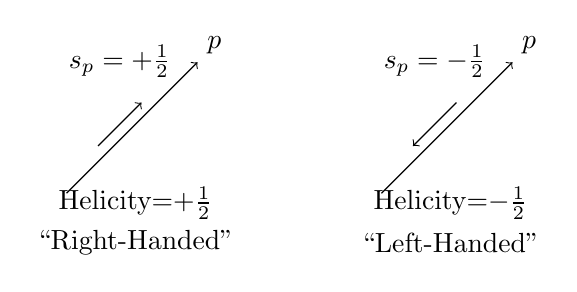
\begin{tikzpicture}[scale=2.0]
    \node (A) at (0,0) {};
    \node (B) at (1,1) {$\vb{p}$};
    \node (Aspin) at (0.4,0.9) {$s_{\vu{p}}=+\frac12$};
    \node (Ap) at (0.2,0.3) {};
    \node (Bp) at (0.6,0.7) {};
    \node (C) at (2,0) {};
    \node (D) at (3,1) {$\vb{p}$};
    \node (Cspin) at (2.4,0.9) {$s_{\vu{p}}=-\frac12$};
    \node (Cp) at (2.2,0.3) {};
    \node (Dp) at (2.6,0.7) {};
    \draw [->] (A) -- (B);
    \draw [->] (Ap) -- (Bp);
    \draw [->] (C) -- (D);
    \draw [<-] (Cp) -- (Dp);
    \node (plus) at (0.5,0) {Helicity=$+\frac12$};
    \node (minus) at (2.5,0) {Helicity=$-\frac12$};
    \node (plusT) at (0.5,-0.25) {``Right-Handed''};
    \node (minusT) at (2.5,-0.25) {``Left-Handed''};
  \end{tikzpicture}
  \caption{Helicity demo}
  \label{fig:helicity}
\end{figure}
The helicity of a \underline{massless} particle is a Lorentz invariant, i.e. the same in all frames: helicity $= \frac12\bm\sigma\vdot\vu{p}$.

Look closer at QCD: It conserves helicity:
\begin{figure}[H]
  \centering
  \begin{tikzpicture}[scale=2.0]
    \begin{feynhand}
      % Symbols
      \vertex (eq) at (1.75,0) {=};
      \vertex (pl) at (3.75,0) {+};
      % vertices
      \vertex (p11) at (1.5,0.5) {$u$};
      \vertex (p12) at (1.5,-0.5) {$\bar{u}$};
      \vertex (a1) at (0,0) {};
      \vertex (b1) at (1,0);
      % propagators
      \propag [gluon] (a1) to (b1);
      \propag (b1) to (p11);
      \propag (b1) to (p12);
      % vertices
      \vertex (p21) at (3.5,0.5) {$u_L$};
      \vertex (p22) at (3.5,-0.5) {$\bar{u}_L$};
      \vertex (a2) at (2,0) {};
      \vertex (b2) at (3,0);
      % propagators
      \propag [gluon] (a2) to (b2);
      \propag (b2) to (p21);
      \propag (b2) to (p22);
      % vertices
      \vertex (p31) at (5.5,0.5) {$u_R$};
      \vertex (p32) at (5.5,-0.5) {$\bar{u}_R$};
      \vertex (a3) at (4,0) {};
      \vertex (b3) at (5,0);
      % propagators
      \propag [gluon] (a3) to (b3);
      \propag (b3) to (p31);
      \propag (b3) to (p32);
    \end{feynhand}
  \end{tikzpicture}
  \caption{QCD Conservation of Helicity}
  \label{fig:qcdhelicity}
\end{figure}
Due to the time conventions, this interation looks like:
\begin{figure}[H]
  \centering
  \begin{tikzpicture}[scale=2.0]
    \begin{feynhand}
      % vertices
      \vertex (u1) at (0,0) {$u_L$};
      \vertex (u2) at (2,0) {$u_L$};
      \vertex (a) at (1,0);
      \vertex (b) at (1,-1);
      % propagators
      \propag [gluon] (a) to (b);
      \propag [mom'={}] (a) to (u1);
      \propag [mom'={}] (u2) to (a);
    \end{feynhand}
  \end{tikzpicture}
  \caption{Equivalent to \ref{fig:qcdhelicity}}
  \label{fig:qcdhelicity2}
\end{figure}
Replacing the $u$ with $d$ gives the same $SU(2)$ structure, except for each of the left and right helicity particles, giving an $SU(2)_L$ and $SU(2)_R$. So the full symmetry of QCD is:
\begin{align*}
  SU(2)_{L}\otimes SU(2)_{R}
\end{align*}
Which better represents the chiral symmetry.

We saw that $SU(2)_{isospin}$ led to three pions of equal mass, ($\pi^+,\pi^0,\pi^-$). But the symmetry of QCD is bigger than $SU(2)_I$; why is it not manifest in the particle spectrum? Because $SU(2)_L\otimes SU(2)_R$ is spontaneously broken! This means we really see $SU(2)_I$ as a ``hidden'' version of $SU(2)_L\otimes SU(2)_R$, that is $SU(2)_L\otimes SU(2)_R\to SU(2)_I$. Since we lose 3 degrees of freedom from this ($SU(2)_L\otimes SU(2)_R$ has 6, $SU(2)_I$ has 3).

Recall scalar field: $\phi\to e^{i\alpha}\phi$ under $U(1)$. Since the symmetry is broken or hidden, the ground state value should not obey this $U(1)$, i.e. it is not at $\phi=0$, so assume:
\begin{align*}
  \ev{\phi}_0&=\frac{v}{\sqrt{2}}\\
  \implies\ev{\phi}_0\to e^{i\alpha}\ev{\phi}_0
\end{align*}
This creates a Goldstone Boson!

For quarks, the chirality means they act as a doublet:
\begin{align*}
  q\equiv\pmqty{u\\d}
\end{align*}
And each left/right doublet acts differently under its own $SU(2)_{L/R}$:
\begin{align*}
  SU(2)_L&: q_L\to U_Lq_L, \bar{q}_L\to\bar{q}_LU_L^\dag\\
  U_L&=e^{i\sigma\alpha_L}\in SU(2)_L\\
  SU(2)_R&: q_R\to U_Rq_R, \bar{q}_R\to\bar{q}_RU_R^\dag\\
  U_R&=e^{i\sigma\alpha_R}\in SU(2)_R
\end{align*}

The QCD force produces a condensate:
\begin{align*}
  \ev{\bar{q}q}_0\neq0\implies \ev{\bar{q}_Lq_R+\bar{q}_Rq_L}\neq 0
\end{align*}
This fact breaks BOTH $SU(2)_L$ and $SU(2)_R$:
\begin{align*}
  \ev{\bar{q}_Lq_R+\bar{q}_Rq_L}\underset{SU(2)_L}{\to}
  \bar{q}_LU^\dag_Lq_R+\bar{q}_RU_Lq_L\\
  \ev{\bar{q}_Lq_R+\bar{q}_Rq_L}\underset{SU(2)_R}{\to}
  \bar{q}_LU_Rq_R+\bar{q}_RU^\dag_Rq_L
\end{align*}
So it appears we have kept neither $SU(2)_L$ nor $SU(2)_R$ on their own. Consider rotation by \underline{both} $U_L$ and $U_R$ at the same time and by the same amount, this means $U_L=U_R$, so we get:
\begin{align*}
  \ev{\bar{q}_Lq_R+\bar{q}_Rq_L}\underset{SU(2)_L\otimes SU(2)_R}{\to}
  \bar{q}_L\underbrace{U^\dag_LU_R}_{\bm{1}}q_R+
  \bar{q}_R\underbrace{U^\dag_RU_L}_{\bm{1}}q_L
  =\ev{\bar{q}_Lq_R+\bar{q}_Rq_L}
\end{align*}
Hence, there is an unbroken combination of $SU(2)_L\otimes SU(2)_R$ with $U=U_L=U_R$ that leaves an $SU(2)$ we call isospin! Chiral symmetry breaking is then represented by $SU(2)_L\otimes SU(2)_R\to SU(2)_I$. There are 3 broken symmetries, which lead to our 3 Goldstone bosons $(\pi^+,\pi^0,\pi^-)$. The 3 unbroken symmetries give the remaining Isospin symmetry.


\subsection{Pion Field Theory}
Effective theory of $SU(2)_L\otimes SU(2)_R\to SU(2)_I$:

This is a model of spin-0 fields which displays chiral symmetry breaking -- also called a \underline{``$\sigma$ model''}.

Consider $\phi=\pmqty{a\\b}$, with $a,b\in\mathbb{C}$, so a complex doublet with \underline{4 degrees of freedom}. The Lagrangian is given by:
\begin{align*}
  \L=\D_\mu\phi^\dag\D^\mu\phi-V(\phi^\dag\phi)
\end{align*}
The Lagrangian is invariant under $\phi\to U\phi$ with $U\in SU(2)$.
In fact, the symmetry is even larger. To see this, think of $\phi$ as a matrix:
\begin{align*}
  \Phi &= \pmqty{a&-b^*\\b&a^*}\\
  \phi^\dag\phi&=\abs{a}^2+\abs{b}^2\\
  \Phi^\dag\Phi&=\pmqty{\abs{a}^2+\abs{b}^2\\&\abs{a}^2+\abs{b}^2}\\
  \implies\frac12\Tr[\Phi^\dag\Phi]&=\abs{a}^2+\abs{b}^2
\end{align*}
So rewrite the Lagrangian in terms of $\Phi$:
\begin{align*}
  \L=\frac12\Tr[\D_\mu\Phi^\dag\D^\mu\Phi]-V\qty(\frac12\Tr[\Phi^\dag\Phi])
\end{align*}
Note that $\det\Phi$ also is $\abs{a}^2+\abs{b}^2$, so we have the constraint that:
\begin{align*}
  \det\Phi=\frac12\Tr[\Phi^\dag\Phi]
\end{align*}
This Lagrangian obeys 2 very different symmetries:
\begin{align*}
  \Phi\to U_L\Phi\quad U_L\in SU(2)_L\\
  \Phi\to \Phi U_R^\dag\quad U_R\in SU(2)_R
\end{align*}

Lets get to the symmetry breaking. Let $\ev{\Phi}_0\neq0$, specifically choose $a=\frac{v}{\sqrt{2}},b=0$, or:
\begin{align*}
  \ev{\Phi}_0=\frac1{\sqrt{2}}\pmqty{v\\&v}
\end{align*}
This is the same story and physics as before, transform this under the combination $SU(2)_L\otimes SU(2)_R$
\begin{align*}
  \ev{\Phi}_0\underset{SU(2)_L\otimes SU(2)_R}{\to}
  U_L\ev{\Phi}_0U^\dag_R=\frac1{\sqrt{2}}\pmqty{v\\&v}U_LU_R^\dag
\end{align*}
We can exchange $\ev{\phi_0}$ and $U_L$ since it is proportional to the identity. This will only go back to $\ev{\Phi}_0$ if $U_L=U_R$, the rotations are by the same amount. This is the isospin again!

As before, consider the shifted field with a zero vacuum expectation value (vev):
\begin{align*}
  \Phi=\frac1{\sqrt{2}}\pmqty{\sigma+v\\&\sigma+v}
  \exp[\frac{i}2\bm{\tau}\vdot\bm{\pi}]
\end{align*}
Where $\tau_i$ are the Pauli Matrices, and $\pi_i$ are the pion fields. Note that $\sigma$ are \emph{not} the pauli matrices, they are another field. This time the potential becomes:
\begin{align*}
  V&=\lambda\qty(\frac12\Tr\Phi^\dag\Phi-\frac{v^2}2)^2\\
  &=\lambda\qty(\frac122\frac12(\sigma+v)^2-\frac{v^2}2)^2\\
  &=\lambda\qty(\frac12\sigma^2+\sigma v)^2
\end{align*}
Notice that the pion fields disappear from the trace due to them being completely in the exponential. This means that $\pi_i$ are massless Goldstone bosons, with ($i=1,2,3$).

Under Isospin, we have:
\begin{align*}
  \Phi&=\frac1{\sqrt{2}}\pmqty{\sigma+v\\&\sigma+v}e^{i/2 \tau\vdot\pi}\\
  U\Phi U^\dag=\frac1{\sqrt{2}}\pmqty{\sigma+v\\&\sigma+v}
  Ue^{i/2\tau\vdot\pi}U^\dag
\end{align*}
The remaining part, $Ue^{i/2\tau\vdot\pi}U^\dag$, can be written as $e^{i/2\tau\vdot\pi'}$, where $\pi_i'$ are rotated $\pi$ fields.

The Physics of the $\sigma$ field is a bit murky. We see it in a broad enhancement in $\pi\pi$ scattering, so we see something like $\pi\pi\to\sigma\to\pi\pi$.

But the $\sigma$ is not in the Particle Data Book, but that just means its existence is not unambiguous. What even is a particle?

\subsection{Strangeness and $SU(3)$}
Lets add the strange quark to the discussion:
\begin{align*}
  \pmqty{u\sim\SI{4}{\MeV}\\d\sim\SI{7}{\MeV}\\s\sim\SI{150}{\MeV}\\}
\end{align*}
The charge of $s$ is $-\frac{1}{3}$, so it is not a triplet of EM, but rather it is a triplet of a new flavor, $SU(3)$. Note that we were able to ignore this quark model and work with the broken chiral symmetry of $SU(2)_I$ since the mass of the $u$ and $d$ were much less than the mass of the constituent particles we were dealing with. So approximating the full QCD as just $SU(3)$ will not be as good of an approximation since $m_s$ is so large. 

Recall that the pions all had $I=1$ and corresponded to the triplet states of adding two $I=1/2$ particles, the missing $I=0$ state involves the strange quark and is the $\eta(547)=\frac1{\sqrt{6}}\qty(u\bar{u}-d(-\bar{d})-2s\bar{s})$. Thus means that the $s$ quark is an isospin singlet.

\subsubsection{New Mesons}
We have a couple new mesons corresponding to our new quark:
\begin{itemize}
\item The $d$ and $\bar{s}$ make a $K^0$, and its antiparticle $-\bar{d}$ and $s$ make a $\bar{K}^0$, with mass \SI{497.6}{\MeV}
\item The corresponding positively charged particle is from the $u$ and $\bar{s}$, the $K^+$, with mass \SI{493.6}{\MeV}
\item The corresponding negatively charged particle is from the $\bar{u}$ and $s$, the $K^-$, with mass \SI{493.6}{\MeV}
\end{itemize}
$K_0$ and $K^+$ form an isospin doublet, as do $\bar{K}^0$ and $K^-$, but how do they $K$'s fit together with the $\pi$'s under $SU(3)$?

\subsubsection{Fundamental Representation of $SU(3)$}
The fundamental representation of $SU(3)$ is $3\times3$ unitary matrix $U=e^{i\theta\vdot T}$ with $\det{U}=1$, this gives 9-1=8 generators $T$. The parameters $\theta\vdot T=\theta^AT^A$, $A=1,\dots,8$. So $SU(3)$ is 8-dimensional, and the 3-dimensional represetation much satisfy the Lie Algebra $\comm{T^A}{T^B}=if^{ABC}T^C$ relation. One such representation is:
\begin{align*}
  T^1&=\frac12\pmqty{0&1&0\\1&0&0\\0&0&0}\quad
  T^2=\frac12\pmqty{0&-i&0\\i&0&0\\0&0&0}\quad
  T^3=\frac12\pmqty{1&0&0\\0&-1&0\\0&0&0}\quad
  T^4=\frac12\pmqty{0&0&1\\0&0&0\\1&0&0}\\
  T^5&=\frac12\pmqty{0&0&-i\\0&0&0\\i&0&0}\quad
  T^6=\frac12\pmqty{0&0&0\\0&0&1\\0&1&0}\quad
  T^7=\frac12\pmqty{0&0&0\\0&0&-i\\0&i&0}\quad
  T^8=\frac1{2\sqrt{3}}\pmqty{1&0&0\\0&1&0\\0&0&-2}
\end{align*}
Notice that the pauli matrices $\sigma$ are embedded inside this larger group. Also notice that $\Tr[T^A]=0$.

This gives us an explicit representation, but the group is identified by the totally antisymmetric structure constants $f^{ABC}$:
\begin{itemize}
\item There are $8\times8\times8=512$ constants here!
\item Of course if $A=B$, $A=C$ or $B=C$, they are 0 by symmetry
\item The non-zero ones are:
  \begin{align*}
    f^{123}&=1\quad(\text{convention})\\
    f^{147}&=f^{246}=f^{257}f^{345}=f^{516}=f^{637}=\frac12\\
    f^{458}&=f^{678}=\frac{\sqrt{3}}{2}
  \end{align*}
  You can get the rest through the antisymmetric property
\end{itemize}
So, the quark triplet $\pmqty{u&d&s}$ is transformed under the fundamental representation given by the $T^A$ above. The antiquark triplet $\pmqty{\bar{u}&\bar{d}&\bar{s}}$ transforms under the complex conjugate representation, $-(T^A)^*$. However unlike $SU(2)$, this representation is not unitarily equivalent to the fundamental representation.
The fundamenetal representation is called a $3$, and its unrelated complex conjugate is a $\bar{3}$
While the quarks and antiquarks transform under 3 and $\bar{3}$, respectively, the $\pi$'s and $K$'s transform under a different representation called the \emph{adjoint} representation.
The adjoint representation must satify the Lie Algebra $\comm{T^A}{T^B}=if^{ABC}T^C$. Think of $(f^A)^{BC}$ as a set of $A=1,\dots,N$ matrices of dimension $N\times N$, (For $SU(3)$, $N=8$). A convenient way to construct the adjoint generators is to choose $(T^A)^{BC}=-if^{ABC}$.

\begin{definition}[Adjoint Representation]
  The dimension of an adjoint representation has the same dimension as the group
\end{definition}
Lets plug in to $\comm{T^A}{T^B}=if^{ABC}T^C$:
\begin{align*}
  (T^A)^{DE}(T^B)^{EF}-(T^B)^{DE}(T^A)^{EF}&=if^{ABC}(T^C)^{DF}\\
  \implies -f^{ADE}f^{BEF}+f^{BDE}f^{AEF}&=f^{ABC}f^{CDF}\\
  \implies f^{ADE}f^{EBF}+f^{BDE}f^{AEF}&+f^{BAE}f^{EDF}=0
\end{align*}
This important relation is called the Jacobi identity. So we have shown these matrices $(T^A)^{BC}$ satisfy the Lie Algebra, and form the adjoint representation.

The $\pi$'s and $K$'s transform as an octet (8) under this representation. This is usually displayed as:
\begin{figure}[H]
  \centering
  \begin{tikzpicture}
    % axes
    \draw[latex-latex, thin, draw=gray] (-2.4,0)--(2.4,0) node [right] {$I$};
    \draw[latex-latex, thin, draw=gray] (0,-2.4)--(0,2.4) node [above] {$s$};
    % positions on axes
    \node at (-0.75, 1.3) {\textbullet};
    \node at (-0.75, 1.3) [above] {\(K^0\)};
    \node at ( 0.75, 1.3) {\textbullet};
    \node at ( 0.75, 1.3) [above] {\(K^+\)};
    \node at (-0.75,-1.3) {\textbullet};
    \node at (-0.75,-1.3) [below] {\(K^-\)};
    \node at ( 0.75,-1.3) {\textbullet};
    \node at ( 1.0,-1.3) [below] {\(\overline{K}^0\)};
    \node at (-1.5, 0.0) {\textbullet};
    \node at (-1.5, 0.0) [below] {$\pi^-$};
    \node at ( 0.0, 0.0) {\textbullet};
    \node at ( 0.0, 0.0) [below] {$\pi^0$};
    \node at ( 1.5, 0.0) {\textbullet};
    \node at ( 1.5, 0.0) [below] {$\pi^+$};
    \node at ( 0.1, 0.1) {\textbullet};
    \node at ( 0.1, 0.1) [above] {$\eta(547)$};
    % strangeness labels
    \node at (-2.9, 0.0) {$s=0$};
    \node at (-2.9, 1.3) {$s=+1$};
    \node at (-2.9,-1.3) {$s=-1$};
  \end{tikzpicture}
  \caption{Strangeness and Isospin Plot}
  \label{fig:strangeisospin}
\end{figure}
We fill out the octet with the $I=0$ meson $\eta(547)$. The $\eta$ mass is dominated by the strange quarks inside.

Note: It is a historical accident that the $s$ quark has $S=-1$, and $\bar{s}$ has $S=1$.

The quark content of each of these is:
\begin{gather*}
  K^+=u\bar{s}\qquad \bar{K}^0=-\bar{d}s\quad K^0=d\bar{s}\quad K^-=\bar{u}s\\
  \eta=\frac1{\sqrt{6}}(u\bar{u}+d\bar{d}-2s\bar{s})
\end{gather*}
Notice the structure of $\eta$'s quark content is similar to the generator $T^8$, similarly, $\pi^0$ is similar to $T^3$ in the fundamental representation. Mesons are $q\bar{q}$, so we have $3\otimes\bar{3}=8\oplus1$. Where the $3$ represents a quark, $\bar{3}$ an antiquark.

Just like $SU(2)_L\otimes SU(2)_R\to SU(2)_I$, we now have a larger $SU(3)_L\otimes SU(3)_R$ being broken, this time to $SU(3)$ and 8 broken generators, where $\pi$, $\kappa$, and $\eta$ are the pseudo-goldstone bosons.
The singlet state is $\eta'(958)=\frac1{\sqrt{3}}(u\bar{u}+d\bar{d}+s\bar{s})$, Why is the mass so large? $\eta'(958)$ is a goldstone boson of $U(1)_{Axial}$, should be ~massless:
\begin{align*}
  q_L\to e^{i\alpha_L}q_L,\quad q_R\to e^{i\alpha_R}q_R\\
  \alpha_L=\alpha_R\implies \text{Baryon Number}\\
  \alpha_L=-\alpha_R\implies \text{Axial $U(1)$}
\end{align*}
This $U(1)_A$ is broken by the vacuum meson state $\ev{\bar{q}q}_0$.

$U(1)_A$ is \emph{not} a symmetry due to a quantum field theoretic anomaly (quantum effects do not preserve the symmetry). This implies $\eta'$ is \emph{not} a goldstone boson. Its mass comes from a topological effect of field configurations called instantons.

\subsubsection{$J=1$ Mesons}

\begin{figure}[H]
  \centering
  \begin{tikzpicture}
    % positions on axes
    \node at (-0.75, 1.3) {\textbullet};
    \node at (-0.75, 1.3) [above] {\(K^{*0}\)};
    \node at ( 0.75, 1.3) {\textbullet};
    \node at ( 0.75, 1.3) [above] {\(K^{*+}\)};
    \node at (-0.75,-1.3) {\textbullet};
    \node at (-0.75,-1.3) [below] {\(K^{*-}\)};
    \node at ( 0.75,-1.3) {\textbullet};
    \node at ( 1.0,-1.3) [below] {\(\overline{K}^{*0}\)};
    \node at (-1.5, 0.0) {\textbullet};
    \node at (-1.5, 0.0) [below] {$\rho^-$};
    \node at ( 0.0, 0.0) {\textbullet};
    \node at ( 0.0, 0.0) [below] {$\rho^0$};
    \node at ( 1.5, 0.0) {\textbullet};
    \node at ( 1.5, 0.0) [below] {$\rho^+$};
    \node at ( 0.1, 0.1) {\textbullet};
    \node at ( 0.1, 0.1) [above] {$\omega_8$};
    % strangeness labels
    \node at (-2.9, 0.0) {$s=0$};
    \node at (-2.9, 1.3) {$s=+1$};
    \node at (-2.9,-1.3) {$s=-1$};
  \end{tikzpicture}
  \caption{Strangeness/Isospin Octet with $J=1$}
  \label{fig:strangeisospin2}
\end{figure}
Note the mass of $K^*(894)$ and $\rho(775)$.

Similar to the $\eta$ with $J=0$, the $J=1$ $\omega_8=\frac1{\sqrt{6}}(u\bar{u}+d\bar{d}-2s\bar{s})$. Much like the $\eta'$, the singlet is $\omega_1=\frac1{\sqrt{3}}(u\bar{u}+d\bar{d}+s\bar{s})$.

In Nature, $\omega_1$ and $\omega_8$ mix. The observed states are:
\begin{align*}
  \omega&=\frac1{\sqrt{3}}\omega_8+\sqrt{\frac23}\omega_1=
  \frac1{\sqrt{2}}(u\bar{u}+d\bar{d})\\
  \phi&=-\sqrt{\frac23}\omega_8+\frac1{\sqrt{3}}=s\bar{s}
\end{align*}
The mass of $\omega(783)$ and $\phi(1020)$.

Notice in these states, the $(u,d)$ and $s$ separate from each other.


\subsubsection{Strange Baryons}
Recall $SU(2)_I$ Baryons, we had $2\otimes2\otimes2=4\oplus 2_S\oplus 2_A$. The $4$ was the $\Delta$.

Perform the same construction for $SU(3)$. Let 3 representations by $\psi^i$ and $\chi^i$, $i=1,2,3$:
\begin{align*}
  3\otimes3=\psi^i\chi^j=
  \underbrace{\frac12\qty(\psi^i\chi^j+\psi^j\chi^i)}_{S^{ij}\text{ Symmetric}}
  +\underbrace{\frac12\qty(\psi^i\chi^j-\psi^j\chi^i)}_{A^{ij}\text{ Antisymmetric}}
\end{align*}
Note that $S^{ij}$ is a $3\times3$ symmetric matrix with 6 independent elements, and $A^{ij}$ is a $3\times3$ antisymmetric matrix with 3 independent elements. This means $3\otimes3=6\oplus\bar{3}$, the $\bar{3}$ is not obvious here.

Add one quark:
\begin{align*}
  3\otimes(3\otimes3)=3\otimes(6\oplus\bar{3})
\end{align*}
Break this into pieces:
\begin{enumerate}
\item $3\otimes6$:
  \begin{align*}
    \psi^kS^{ij}&=\frac12\qty(\psi^kS^{ij}+\psi^iS^{kj}+\psi^jS^{ik})
    +\frac12\qty(\psi^kS^{ij}-\psi^iS^{kj}-\psi^jS^{ik})\\
    &=S^{kij}+M^{kij}
  \end{align*}
  Where $S^{ijk}$ is a totally symmetric matrix, with 10 independent elements, and $M^{kij}$ is symmetric only on $i\iff j$, so $8$ independent elements.

  The end result is $3\otimes 6=10\oplus 8$
\item $3\otimes\bar{3}=8\oplus 1$ we know from mesons
\end{enumerate}
Thus we get $3\otimes 3\otimes 3=10_s\oplus8_M\oplus8_M\oplus1$, a decuplet, 2 octets, and a singlet.
\begin{figure}[H]
  \centering
  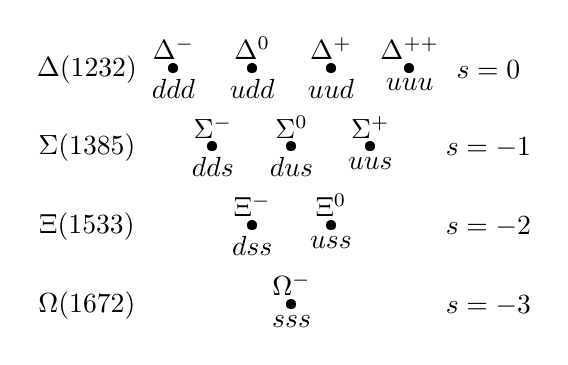
\begin{tikzpicture}
    % labels for each particle
    \node at ( 0.0, 3.0) {$\Delta(1232)$};
    \node at ( 0.0, 2.0) {$\Sigma(1385)$};
    \node at ( 0.0, 1.0) {$\Xi(1533)$};
    \node at ( 0.0, 0.0) {$\Omega(1672)$};
    % s=0 Deltas
    \node at ( 1.1, 3.0) {\textbullet};
    \node at ( 1.1, 3.0) [above] {$\Delta^-$};
    \node at ( 1.1, 3.0) [below] {$ddd$};
    \node at ( 2.1, 3.0) {\textbullet};
    \node at ( 2.1, 3.0) [above] {$\Delta^0$};
    \node at ( 2.1, 3.0) [below] {$udd$};
    \node at ( 3.1, 3.0) {\textbullet};
    \node at ( 3.1, 3.0) [above] {$\Delta^+$};
    \node at ( 3.1, 3.0) [below] {$uud$};
    \node at ( 4.1, 3.0) {\textbullet};
    \node at ( 4.1, 3.0) [above] {$\Delta^{++}$};
    \node at ( 4.1, 3.0) [below] {$uuu$};
    % s=-1 sigma
    \node at ( 1.6, 2.0) {\textbullet};
    \node at ( 1.6, 2.0) [above] {$\Sigma^-$};
    \node at ( 1.6, 2.0) [below] {$dds$};
    \node at ( 2.6, 2.0) {\textbullet};
    \node at ( 2.6, 2.0) [above] {$\Sigma^0$};
    \node at ( 2.6, 2.0) [below] {$dus$};
    \node at ( 3.6, 2.0) {\textbullet};
    \node at ( 3.6, 2.0) [above] {$\Sigma^+$};
    \node at ( 3.6, 2.0) [below] {$uus$};
    % s=-2 cascade
    \node at ( 2.1, 1.0) {\textbullet};
    \node at ( 2.1, 1.0) [above] {$\Xi^-$};
    \node at ( 2.1, 1.0) [below] {$dss$};
    \node at ( 3.1, 1.0) {\textbullet};
    \node at ( 3.1, 1.0) [above] {$\Xi^0$};
    \node at ( 3.1, 1.0) [below] {$uss$};
    % s=-3 omega
    \node at ( 2.6, 0.0) {\textbullet};
    \node at ( 2.6, 0.0) [above] {$\Omega^-$};
    \node at ( 2.6, 0.0) [below] {$sss$};
    % Strangeness labels
    \node at ( 5.1, 3.0) {$s= 0$};
    \node at ( 5.1, 2.0) {$s=-1$};
    \node at ( 5.1, 1.0) {$s=-2$};
    \node at ( 5.1, 0.0) {$s=-3$};
  \end{tikzpicture}
  \caption{Baryon Decuplet $J=\frac32$}
  \label{fig:decuplet}
\end{figure}
Remember, states are symmetrized, e.g.: $\Sigma^0=(dus+dsu+uds+usd+sud+sdu)/\sqrt{6}$.

Also as an aside, the $\Xi$ is not ``xi'' but rather ``cascade''

\begin{figure}[H]
  \centering
  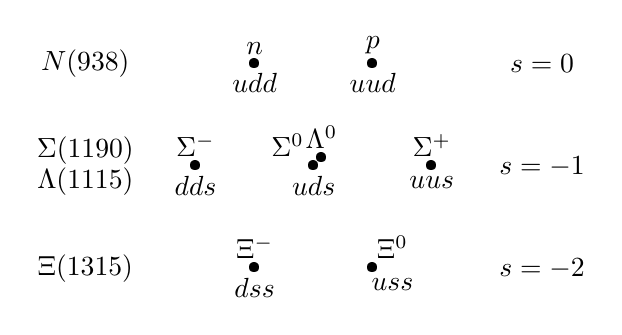
\begin{tikzpicture}
    % positions on axes
    \node at (-0.75, 1.3) {\textbullet};
    \node at (-0.75, 1.3) [above] {$n$};
    \node at (-0.75, 1.3) [below] {$udd$};
    \node at ( 0.75, 1.3) {\textbullet};
    \node at ( 0.75, 1.3) [above] {$p$};
    \node at ( 0.75, 1.3) [below] {$uud$};
    \node at (-0.75,-1.3) {\textbullet};
    \node at (-0.75,-1.3) [above] {$\Xi^-$};
    \node at (-0.75,-1.3) [below] {$dss$};
    \node at ( 0.75,-1.3) {\textbullet};
    \node at ( 1.0,-1.3) [above] {$\Xi^{0}$};
    \node at ( 1.0,-1.3) [below] {$uss$};
    \node at (-1.5, 0.0) {\textbullet};
    \node at (-1.5, 0.0) [above] {$\Sigma^-$};
    \node at (-1.5, 0.0) [below] {$dds$};
    \node at ( 0.0, 0.0) {\textbullet};
    \node at ( 0.0, 0.0) [above left] {$\Sigma^0$};
    \node at ( 0.0, 0.0) [below] {$uds$};
    \node at ( 1.5, 0.0) {\textbullet};
    \node at ( 1.5, 0.0) [above] {$\Sigma^+$};
    \node at ( 1.5, 0.0) [below] {$uus$};
    \node at ( 0.1, 0.1) {\textbullet};
    \node at ( 0.1, 0.1) [above] {$\Lambda^0$};
    % particle labels
    \node at (-2.9, 1.3) {$N(938)$};
    \node at (-2.9, 0.2) {$\Sigma(1190)$};
    \node at (-2.9,-0.2) {$\Lambda(1115)$};
    \node at (-2.9,-1.3) {$\Xi(1315)$};
    % strangeness
    \node at (2.9, 1.3) {$s= 0$};
    \node at (2.9, 0.0) {$s=-1$};
    \node at (2.9,-1.3) {$s=-2$};
  \end{tikzpicture}
  \caption{Baryon Octet $J=\frac12$}
  \label{fig:octet}
\end{figure}
These states must be symmetrized in flavor an spin (like $p,n$). Generally you just replace $u,d$ with $s$. $\Sigma^0$ can be found from $\Sigma^-$ via isospin; $\Lambda^0$ is orthogonal to $\Sigma^0$.

Note: Do not confuse the $J=\frac32$ particles with the $\frac12$ ones, despite their names being similar, they are different.

\subsection{Beyond $SU(3)$}
Adding a charm quark $c$ leads to an $SU(4)$, see Particle Data Group. While the symmetry increases, but now badly broken. If $m_c\sim\SI{1.5}{\GeV}$, this is comparable to hadron masses.

Adding the bottom quark $b$ gives $SU(5)$, $m_b\sim\SI{4.5}{\GeV}$. The $b$ baryons found in 2006, $\Sigma_b(5810), \Sigma_b^*(5830)$, then in 2007, the $\Xi^-_b(5793)$

Adding a top quark does NOT give $SU(6)$, but $m_t\sim\SI{175}{\GeV}$. The top quark decays before it can hadronize.

There are a lot of other possible states -- orbital and/or radial excitations of those we've explored.

There also appear to be ``exotics'': E.g. $f_0(980)$ is believed to be a $K\bar{K}$ bound state (``molecule''), as its mass is very close to $2m_K=\SI{990}{\MeV}$. There was lots of excitement about possible ``pentaquark'' states -- $qqqq\bar{q}$, they seemed too narrow (width) for molecuules, but really were baryons and mesons very close.

There have been many statistically ``significant'' exotics identified over the years ... many have gone away.

\subsection{Beyond Stamp Collectings}

\subsubsection{Masses}
How do we find quark masses?
\begin{enumerate}
\item $\frac{m_\pi^2}{m_K^2}=\frac{ud}{us}$ This gives an estimate for the ratio of the first generation ($u,d$) quarks average mass to the mass of the strange.
\item We can use measurements of the $\Delta^{++}$ and $\Sigma^+$ to get measurements of the strange mass since it would clearly dominated by the strange, so $m_s\sim\SI{150}{\MeV}$
\item We can then get that the average mass of $u,d$ should be $\SI{6}{\MeV}$
\item We can then use the mass measurements of the $K^0$ and $K^+$ to get the ratio of the $u/d$, and find that $m_u\sim\SI{4}{\MeV}$ and $m_d\sim\SI{7}{\MeV}$
\end{enumerate}

We can estimate $m_c$ and $m_b$ best from heavy-quark effective theory (HQET) and now lattice QCD calculations.

$m_t$ can be directly reconstructed from decay products.

\paragraph{Hadron masses} For hadrons with zero orbital angular momenta, the interaction between quarks can depend on the relative orientation of their spins. An empirical expression for meson and baryon masses is:
\begin{align*}
  M_{\text{meson}}&=m_1+m_2+a\frac{\bm{\sigma}_1\vdot\bm{\sigma}_2}{m_1m_2}\\
  M_{\text{baryon}}&=m_1+m_2+m_3+\frac{a'}{2}\sum_{i>j}
  \frac{\bm{\sigma}_i\vdot\bm{\sigma}_j}{m_im_j}
\end{align*}
The dot product $\bm{\sigma}_i\vdot\bm{\sigma}_j$ is the QCD analog of the ``hyperfine'' interaction in QED.

For mesons:
\begin{align*}
  \bm{\sigma}_1\vdot\bm{\sigma}_2&=4(\vb{s}_1\vdot\vb{s}_2)
  =2\qty[(\vb{s}_1+\vb{s}_2)^2-\abs{\vb{s}_1}^2-\abs{\vb{s}_2}^2]\\
  &=2\qty[s(s+1)-s_1(s_1+1)-s_2(s_2+1)]=2\qty[s(s+1)-\frac32]=
  \begin{cases}
    1 & s=1 \\ -3 & s=0
  \end{cases}
\end{align*}
Assuming constituent $m_u=m_d=\SI{310}{\MeV}$, $m_s=\SI{483}{\MeV}$ and $a=\SI{160}{\MeV}$, we get the following calculated masses:
\begin{table}[H]
\centering
\begin{tabular}{c|cccccc}
(\si{\MeV}) & $\pi^\pm$ & $\rho$ & $K$ & $K^*$ & $\eta$ & $\phi$ \\ \hline
Calculated  & 140       & 780    & 484 & 890   & 559    & 1032   \\
Observed    & 140       & 776    & 495 & 892   & 549    & 1020  
\end{tabular}
\caption{Calculated vs. Observed Masses}
\label{tab:obs-vs-calc}
\end{table}

\subsubsection{Magnetic Dipole Moments of Hadrons}
Magnetic dipole moment $\bm{\mu}=\frac{Qe}{2m}g\vb{s}$, $m$ is mass, $\vb{s}$ is spin. From Dirac theory for spin-$\frac12$ particles, $g=2$.

For quarks: $\mu_u=\frac{e\hbar}{3m_uc}$, $\mu_d=-\frac{e\hbar}{6m_dc}$, the magnetic moments for the antiparticles are the negative of these.

For Baryons, $\bm{\mu}_B=\sum_{i}\bm{\mu}_i$.

Recall the structure of the up spin proton:
\begin{align*}
  \ket{p\up}&=\frac1{\sqrt{18}}\qty{
    \qty[2u\up u\up d\dn-u\up u\dn d\up-u\dn u\up d\up]+\dots}\\
  \mu_p&=\frac1{18}\qty{4(\mu_u+\mu_u-\mu_d)
    +(\mu_u-\mu_u-\mu_d)+(\mu_u-\mu_u+\mu_d)}\times 3\\
  &=\frac16\qty[8\mu_u-4\mu_d+2\mu_d]=\frac13[4\mu_u-\mu_d]
\end{align*}
We can similarly find $\mu_n$, or just realize from isospin that $\mu_n=\frac13\qty[4\mu_d-\mu_u]$.

If we assume $m_u=m_d$, the $\mu_d=-\frac12\mu_u$, and we predict that $\mu_n/\mu_p=-2/3$.

Experimentally, we find $\mu_p=2.793\qty(\frac{e\hbar}{2m_pc})$ and $\mu_p=-1.913\qty(\frac{e\hbar}{2m_pc})$, so the ratio is $-0.685$, very close to $-2/3$

